\documentclass[11pt]{article}

\usepackage{amsmath, amsfonts,amssymb,amsthm}
\usepackage{fullpage}
\usepackage{graphicx}

\DeclareGraphicsExtensions{.pdf,.png,.jpg}

\title{6.035 Project 4 Writeup}
\author{Kyle Miller, Alec Thomson, Patrick Hulin, Steven Valdez}
\begin{document}
\maketitle

\section {Instructions for Building and Running the Project}


\section {Overview}

For the final optimization project of our compiler, we decided to
implement two major optimizations and some number of smaller
optimizations. The major optimizations we implemented were Register
Allocation (Section~\ref{sec:regalloc}) and Loop Parallelization
(Section~\ref{sec:parallel}). While these optimizations provided the
most powerful speedups, smaller optimizations we implemented include
Algebraic Simplification (Section~\ref{sec:algebra}), Conditional
Branch Elimination (Section~\ref{sec:condelim}), Expression
Unflattening (Section~\ref{sec:unflat}), Tailcall
Optimizations (Section~\ref{sec:tailcall}), and Assembly Level
Constant and Copy Propagation. Optimizations we wrote for the previous
project including Global Common Subexpression Elimination, Global Copy
Propagation, Constant Propagation, and Unreachable Code Elimination
were all included along with the rest of our optimizations. The design
and implementation of all of our new optimizations is described
below. 

Along with all the optimizations we implemented, we also maintained a
detailed test system (Section~\ref{sec:test}) that helped assure us
of the correctness of our optimizations. Finally, the order and degree
to which we applied the optimizations was important to the
effectiveness of our optimizations and is discussed in Section~\ref{sec:order}.

\section {Division of Work}

The work was divided as follows: Kyle Miller designed and implemented
the register allocator along with a slew of peephole optimizations
that occurred at the code generation level. Kyle also wrote part of
the code generator portion of the loop parallelizer and wrote web
analysis for the Mid-IR that was essential for loop analysis. Alec Thomson wrote most of
the loop analysis routines, including all of the loop parallelization
analysis, the dominator analysis, the loop nesting analysis, and
several loop heuristics that were used by the register allocator and
code generator. Alec
also wrote the expression unflattener to aid with instruction
selection. Patrick Hulin helped write a portion of the loop
parallelizing code generator, wrote some loop invariant code analysis
that ultimately didn't make it in to the final product, and helped
manage the considerable test-suite. Steven Valdez wrote an expression
optimization involving elimination of conditional statements and also
helped manage the test-suite. 

\section{Assumptions}

The following assumptions were made about the Decaf specification.
All of them are arbitrary, and so we feel no need to justify them.
\begin{itemize}
\item The array index expression is evaluated before the assignment
  expression.
\item Binary operators are evaluated left to right.
\item Loop bounds are evaluated from left to right.
\item Method arguments are evaluated right to left.  This was chosen
  when we still used \texttt{push} for stack-based arguments.
\end{itemize}

We assumed a stack-based calling convention in that the stack may
overflow during a call.  However, we did not require stack-based
semantics for method invocation.  For instance, with tail-call
elimination, some programs which would have overflowed the stack were
transformed into programs which no longer did so.  The reason we
assumed stack-based calling semantics was for its straightforwardness
as well as to be able to use C calling conventions for
\texttt{callout}s.

We assumed that division by zero is a run time error in addition to
the array bounds checking and control-flow falloff checking.
Furthermore, we required that a program which failed due to a division
by zero never be transformed into a program which did not fail in such
a manner.  This assumption is required to reason about transformations
like dead code elimination which may remove divisions.  We made this
assumption for consistency: whether a program fails should not be
contingent on whether we performed dead code elimination.  This may
seem contradictory to letting tail call optimization to remove stack
overflows, but stack-based semantics are not part of Decaf (one could
imagine a heap-based calling convention, for instance), but division
semantics are implicitly imported into Decaf by virtue of having
division.

The specification is contradictory as to what may be passed as an
argument to a callout.  At some point it mentions that arrays may be
passed to callouts.  The semantics we chose were that arrays without
square brackets evaluate to the pointer to the first element of the
array.  Furthermore, we assumed that an array is a contiguous block of
$8n$ bytes, where $n$ is the size of the array.  We chose this
convention because it was easy to generate code to interface with such
a convention, and because then the arrays could be passed to callouts
assuming C conventions on the arrays.

The specification was unclear on scoping rules.  We decided on the
following scoping rules.  Scopes are nested, with the global scope as
its root.  There is a method scope for each method with the global
scope as its parent scope.  Each method scope contains as bindings the
formal parameters to the method.  Each block and \texttt{for} loop
defines a new scope, lexically nested.  There may not be multiple
bindings with the same name in any given scoping level.  These rules
admit the following program:
\begin{verbatim}
class Program {
  int x;
  void f(int x) {
    int x;
  }
  void main() { }
}
\end{verbatim}
The specification states that ``the method scope consists of names of
variables and formal parameters introduced in the method declaration''
as well as that ``additional scopes exist within each
$\langle$block$\rangle$ of code''.  But, since a method definition has
no variables, and because the grammar says that the declaration is
followed by a $\langle$block$\rangle$, this means that a method scope
has no variable names in addition to its formal parameters.
Therefore, we accept the above program as valid.  This assumption is
contrary to the assumptions in one of the semantic test cases.

\section{Intermediate Representations}

Our compiler mainly uses two intermediate representations which we
call the mid-IR and the low-IR.  The mid-IR looks roughly like what we
used regularly in class, which consists of expressions, assignments,
and branches. The low-IR is essentially assembly in a control flow
graph.

The various IRs are all instances of control flow graphs parameterized
by the types of instructions found in the graph.  The graphs
themselves are composed of \texttt{Block}s, which are tree-like data
structures consisting of the instructions at their leaves, and which
have the constraint that a label instruction occurs at the beginning
of the block, a jump-like instruction occurs at the end, and neither
such kinds of instructions occur in the middle.

The mid-IR has side-effect-free expression trees contained in possibly
side-effect-full instructions, where the instructions are the leaves
in the \texttt{Block} structures.  We chose this distinction to ensure
that optimizations such as dead code elimination could remove
instructions which were determined to be side-effect-free without
having to inspect the contained subexpressions.

As a consequence to this distinction, division was implemented as an
instruction instead of as an expression because there was the
possibility for division to kill the program with a divide-by-zero
error.  We contemplated adding a division expression for those
divisions which were proved to never divide by zero, but we never got
around to implementing an analysis which would make this useful.

Because the program has been semantically checked before it is
converted to the mid-IR representation, we could simplify the type
system and assume that 64-bit integers were the only type, using C
conventions for booleans.  This simplification reduced the complexity
of the intermediate representations because we had to deal with fewer
kinds of instructions and because we did not have to keep track of
type information.

In the low-IR, there was a data constructor for each kind of assembly
instruction.  We had the type system enforce the constraints on the
kinds of operands which were accepted by the instruction.  For
instance, there were three constructors for the \texttt{mov}
instruction: \texttt{MovIRMtoR}, \texttt{MovIRtoM}, and
\texttt{Mov64toR}.  These correspond to various combinations of moving
immediates, registers, and memory.  The last is a special 64-bit
instruction which moves a 64-bit rather than 32-bit literal into a
register.  This type enforcement prevented us from making mistakes
when constructing assembly in the code generator.

Because the graph is parameterized by the type of instruction, we are
able to perform analyses which are agnostic to the particular kind of
instruction in the graph.  Dominator analysis, liveness analysis, and
web construction could occur on ethir representation because of this.

\section {Algebraic Simplification} 
\label{sec:algebra}

Algebraic simplification occurs on the instructions and expressions in
the mid-IR.  The algebraic simplifier also does constant folding.  We
relied upon the algebraic simplification to put expressions into a
``normal form'' so that the code generator could rely on certain
assumptions.  For instance, we ensured that sums of multiple terms
were always right-associated, and that literals always on the left
side of an addition.

The simplifier itself is structured as a pattern-matching rule system
which recursively rewrites the expression tree from the leaves towards
the root, and restarting this process with the resulting subtree.

Instructions are simplified by simplifying their expressions and then
rewriting the instruction with the new expressions.  The
\texttt{CondBranch} instruction also, in addition, checks if the
conditional expression is a literal and rewrites the instruction into
being a \texttt{Branch} if appropriate.

The following is an example of some rules from the expression
simplifier for binary operations in particular.
{\footnotesize
\begin{verbatim}
simpBinOp :: Ord v => SourcePos -> BinOp -> Expr v -> Expr v
          -> AM (Expr v)
simpBinOp pos op sex1 sex2 = msum rules
    where
      rules =
          [ -- This rule does constant folding if both sides are
            -- constants. (there is no division operation).
            -- Muchnick R1,R3,R5
            do Lit _ i1 <- withExpr sex1
               Lit _ i2 <- withExpr sex2
               return $ Lit pos (binOp op i1 i2)
          -- The following rule enforces the order that literals occur
          -- at the beginning of a sequence of
          -- additions or multiplications
          -- Muchnick R2,R4
          , do guard $ op `elem` [OpAdd, OpMul]
               guard $ sex1 > sex2
               simpES $ BinOp pos op sex2 sex1
          -- Reassociates left-association to right-association for
          -- addition and multiplication while reordering the three
          -- expressions.
          -- backwards Muchnick R7,R8
          , do guard $ op `elem` [OpAdd, OpMul]
               BinOp _ op' oper1 oper2 <- withExpr sex1
               guard $ op' == op
               guard $ oper2 > sex2
               let [a, b, c] = sort [oper1, oper2, sex2]
               oper1' <- simpES $ BinOp pos op a b
               simpES $ BinOp pos op oper1' c
          -- Pulls a constant from the right branch into the left
          -- branch if the left is a constant, too
          -- Backwards muchnick R9, R10
          , do guard $ op `elem` [OpAdd, OpMul]
               Lit litpos i1 <- withExpr sex1
               BinOp _ op' (Lit _ i2) sex2_2 <- withExpr sex2
               guard $ op == op'
               simpES $ BinOp pos op (Lit litpos (binOp op i1 i2)) sex2_2
          -- Reorders the tree if the right-side's left branch is less
          -- than the left branch
          , do guard $ op `elem` [OpAdd, OpMul]
               BinOp pos2 op' sex2_1 sex2_2 <- withExpr sex2
               guard $ op == op'
               guard $ sex1 > sex2_1
               simpES $ BinOp pos op sex2_1 (BinOp pos2 op sex1 sex2_2)
          -- Adding a negation is the same as just subtracting
          , do guard $ op == OpAdd
               UnOp pos1 OpNeg nsex1 <- withExpr sex1
               simpES $ BinOp pos1 OpSub sex2 nsex1

          ...]
\end{verbatim}}

The simplification computation occurs in \texttt{AM}, which is the
\textbf{a}lgebraic simplification \textbf{m}onad.  This is basically
the the \texttt{Maybe} monad, and this is what makes the
\texttt{guard} statements go to the next computation in the
\texttt{msum}.

\section {Expression Unflattener}
\label{sec:unflat}

The purpose of the expression unflattener is to return the mid-ir to
``Tree-Form'' after CSE is performed while maintaining the benefits
gained from CSE so that optimized Instruction Selection can be easily
performed by the code generator. The design, implementation, and test
plan of the unflattener are described below.

\subsection{Design of Expression Unflattener}

Our design first makes use of the liveness information
provided by dead-code elimination to determine which variables are
live at any given block in the mid-ir control flow graph. Once this
information is obtained, unflattening can be performed at the block
level.\\


\noindent Each block is then re-written according to the following algorithm: 

\begin{verbatim}
UnflattenBlock(block):

1. Determine the number of uses of each variable in this block 
2. Determine the reaching definitions of each variable defined in this
block
3. For each variable of each expression in this block: 
   1. If the variable is not live at any of this blocks successors 
      AND the variable is only used once in this entire block 
      (i.e. this is the only use)
      AND the variable is mapped to a reaching definition from this block 
   4. THEN replace the use of this variable with the expression from
its reaching definition
\end{verbatim}

\noindent The UnflattenBlock function is run on the same block until that block
reaches a fixed point. The general purpose of this algorithm is to
discover variables that are ``temporary'' in a given block and to replace
their uses with the expressions they were assigned to represent during
the flattening phase. Since the algorithm doesn't consider a variable
``temporary'' if it is used more than once (or if it is live in a
successor of this block), the benefits of CSE should be preserved
while the mid-ir is returned to tree-form. 

\subsection{Implementation of Expression Unflattener}

The expression unflattener is implemented in the Dataflow.hs source
file. The algorithm is roughly the same as the one described above
with some augmentations to allow for easy fixed point detection.

The first thing the implementation does is use the Hoopl liveness
analysis implemented as part of the previous project to obtain a
factbase of the live variables at the start of every block. Next it
maps the ``UnflattenBlock'' function across every block in the graph
to obtain a new graph with every block flattened to a fixed point. The
``UnflattenBlock'' function will call itself recursively if it detects
that it is returning a changed graph as a result of its
modifications. When ``UnflattenBlock'' no longer has an effect, the
algorithm terminates.

After unflattening every block in the graph, the algorithm then
concludes by performing dead code elimination again to eliminate
assignments to temporaries that are no longer being used.

\subsection{Experimental Results of Expression Unflattener}

The unflattener passes our entire test suite and appears to work
correctly. The figures below show the unflattener operating on a
simple program. The second figure shows how the unflattener maintains
the benefits obtained from CSE. 

\begin{center}
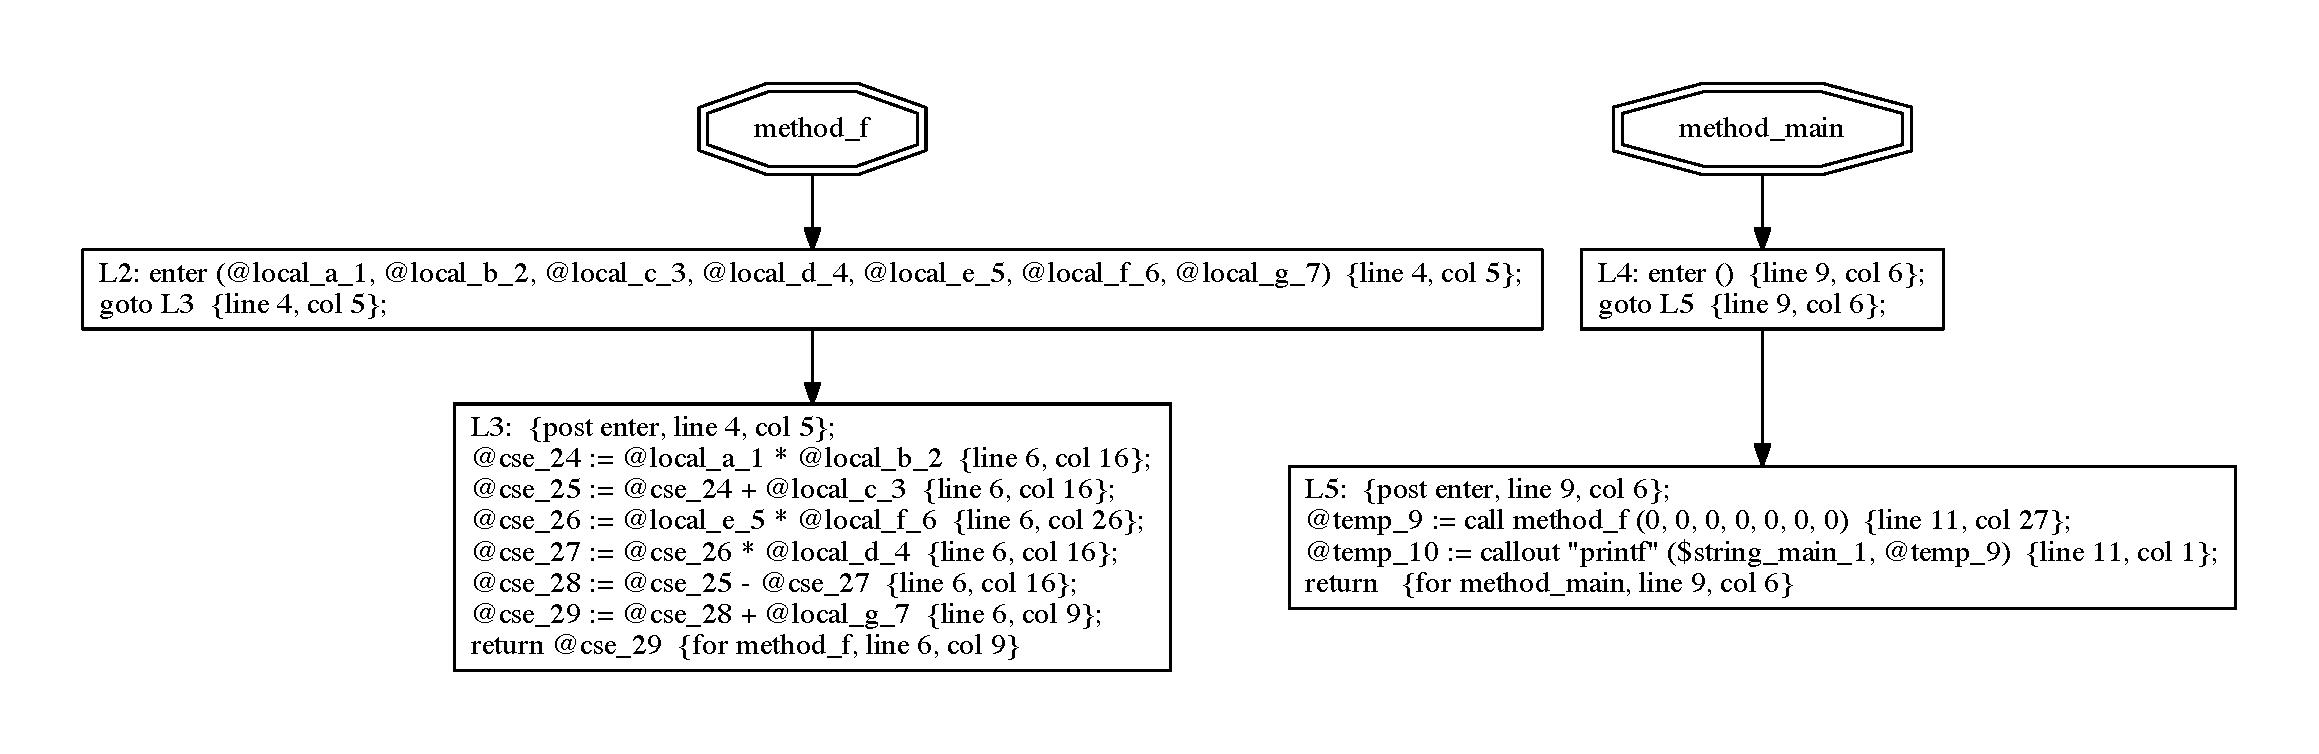
\includegraphics[width=500px]{graphs/unflatten_before}\\
The Mid-IR before unflattening 
\end{center}

\begin{center}
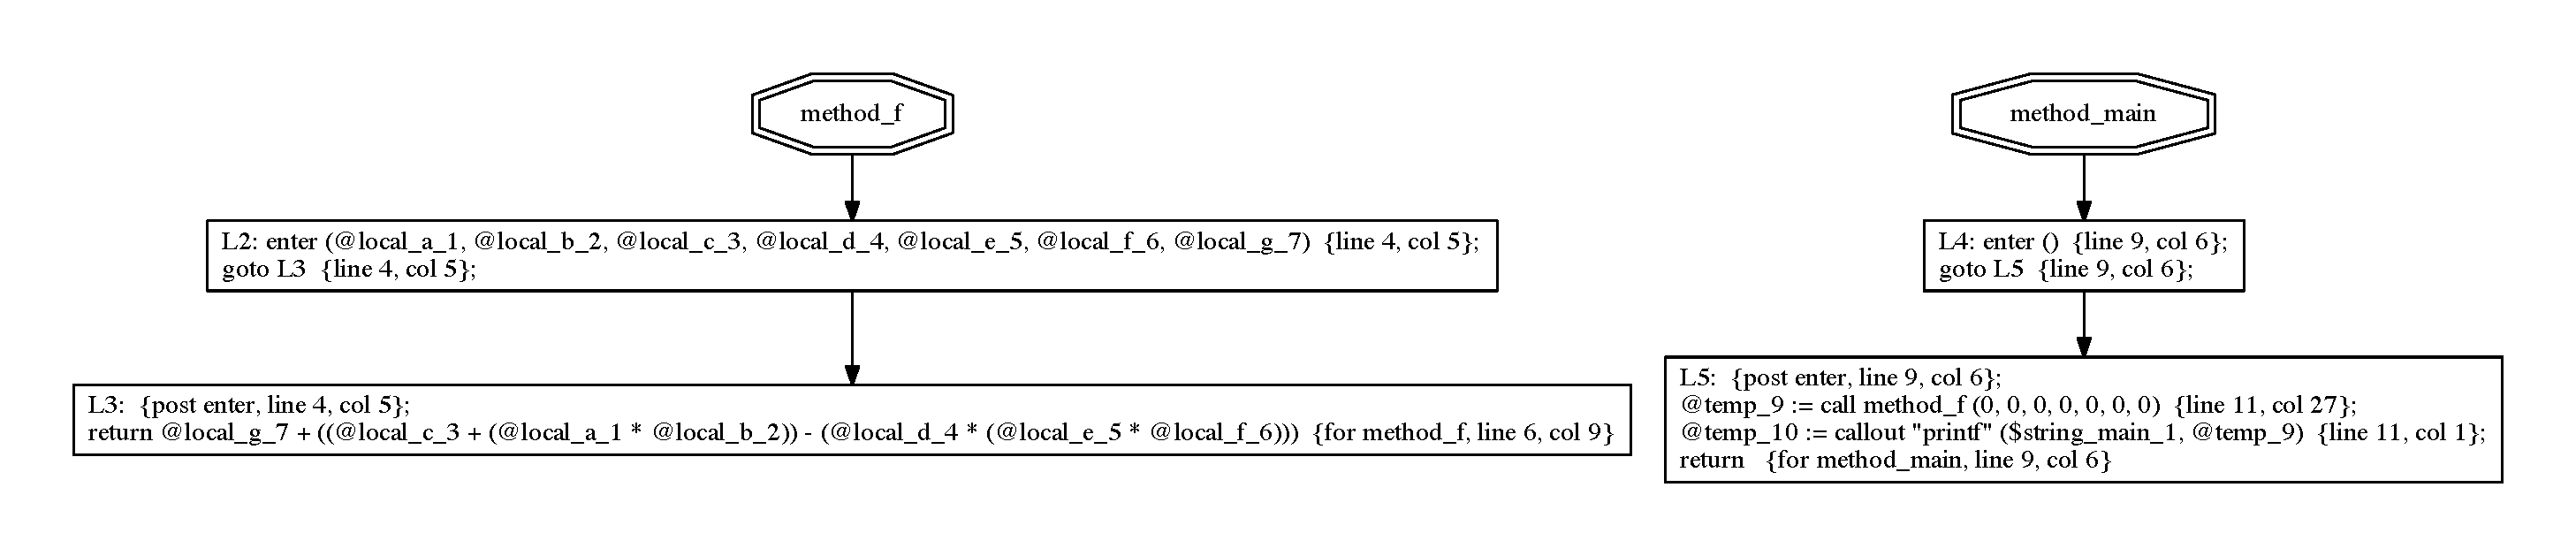
\includegraphics[width=500px]{graphs/unflatten_after}\\
The Mid-IR after unflattening
\end{center}

% TODO: Put the before and after graphs right here for unflattentest1 and unflattentest2

\section {Conditional Elimination} 
\label{sec:condelim}

The conditional eliminator takes \texttt{if} statements whose branches
are simple assignments and rewrites them to be conditional stores.
The conditional eliminator has been disabled in the shipped compiler
because it in certain circumstances made our fixed point computations
use infinite memory.  It was demonstrated to be able to take code such
as:
\begin{verbatim}
int min(int a, int b) {
  if(a < b) {
    return a;
  } else {
    return b;
  }
}
\end{verbatim}
and transform it to be
\begin{verbatim}
int min(int a, int b) {
  return ((a < b) ? a : b);
}
\end{verbatim}
which in the output assembly after register allocation looked like
\begin{verbatim}
min:
  mov %rsi, %rax
  cmpq %rsi, %rdi
  cmovltq %rdi, %rax
  ret
\end{verbatim}
rather than
\begin{verbatim}
min:
  mov %rsi, %rax
  cmp %rsi, %rdx
  jlt L0
  ret
L0:
  mov %rdi, %rax
  ret
\end{verbatim}

This saves a costly jump instruction.

\section {Tailcall Optimization} 
\label{sec:tailcall}

\section {Register Allocation}
\label{sec:regalloc}

We mainly followed the paper ``Iterated Register Coalescing'' by Lal
George and Andrew Appel, which itself based on the Briggs and Chaitlin
algorithms.  We performed the register allocation at our low
intermediate representation, which was essentially assembly.

The first thing which needed to be done was to make it so we could
refer to particular program points.  Our intermediate representations
are built with tree-based blocks, and Haskell makes no distinction
between a pointer to an object and the object itself (that is, there
is no reference-checking equality in Haskell).  What we did was make
an intermediate representation wrapper which added unique ids to each
instruction in the control flow graph.

With these pointers, we could construct DU chains, and with these,
webs.  The DU chains are constructed with a basic backwards dataflow
analysis.  With the chains, we constructed the webs using an algorithm
which kept track of two maps: one of uses at each program point, and
one of definitions at each program point.  The DU chains are inserted
into each of these maps, and when a DU chain is being inserted into a
one of these maps at a program point which already has a DU chain,
then it becomes an alias of the old DU chain.

The interference graph of the webs is constructed over the course of a
backwards dataflow analysis.  An edge between webs is inserted
whenever a definition coincides with the live range of another web.
However, we have added a special case for stores of the form \texttt{x
  := y} which prevents the copy from introducing an interference edge
between the webs for \texttt{x} and \texttt{y}.  This allows the
register allocator to perform the equivalent of copy propagation,
using fewer registers.

\section{Loop Parallelizer}
\label{sec:parallel}

The loop parallelizer splits the control flow into multiple threads
for loops with expensive bodies with no inter-run dependencies. The
analysis runs at the mid IR level 

The design of the loop parallelizer is split into two major parts,
loop analysis and code generation. The loop analysis portion is
concerned with discovering loops that can be parallelized while making
no transformations to the IR. The loop analysis portion is also
responsible for running a heuristic that determines whether loops
should be parallelized considering the overhead of thread
creation. The code generation portion uses the analysis information to 
generate appropriate code to split the loops among many different
threads.

\subsection { Loop Analysis } 

Loop analysis is a multi-stage process that operates on the mid IR
after most of the Mid IR dataflow transformations have completed. We
chose to operate on the Mid IR because it allowed us to parallelize
for-loops and while-loops equally while reaping the full benefits of
constant and copy propagation. The major stages of loop analysis,
described in detail below, are Dominator Analysis, Loop
Identification, Induction Variable Identification, Loop Invariance
Analysis, Cross Dependency Analysis, and Loop Cost
Analysis. Ultimately, the analyzer uses the integer programming method
with the help of the glpk-hs library to solve the cross dependency
constraints.

\subsubsection {Dominator Analysis} 

A useful first step in performing loop analysis was to discover the
dominator map of the midir. To do so, we used a simple forwards
dataflow analysis using Hoopl. The fact type was a set of dominators
while the join function was set intersection with bottom being
represented by the abstract ``Bot'' type. 

The transfer function was very simple and only updated the set of
dominators at entry and exit points of the blocks. Ultimately, Hoopl
took care of most of the analysis and there was no need to rewrite any
portion of the graph. 

The dominator map produced by this analysis was then a map from
block labels to the sets of dominators of those blocks. The dominator
map proved essential to the discovery of loops, loop induction
variables, and loop invariant expressions and variables. 

\subsubsection {Loop Identification}

Once dominator analysis was complete, loops could be identified by
what Muchnick refers to as a ``Back-Edge''. A back-edge is any edge in
the control flow graph that points from a block (referred to as the
``loop-back'' in our code) to one of its dominators (referred to as
the ``loop-header''). Once a back-edge has been identified, the body
of the ``Natural Loop'' can be found by looking for all of the blocks
that are capable of reaching the loop-back \emph{without} travelling
through the loop-header.  

To find all of the blocks in the loop body, another custom dataflow
analysis was performed called ``loop-reaching'' analysis that
ultimately identified all the blocks in the control-flow graph that
could reach the loop-back without travelling through the
loop-header. This was a backwards dataflow analysis with a boolean
fact type that returned the set of blocks belonging to the natural
loop body. 

After the body of the natural loop was discovered, additional blocks
needed to be added to the loop body that were not caught by the
reaching analysis. These blocks were those that ended in return or
fail statements and thus wouldn't be identified as part of the natural
loop but should be considered to be part of the loop body. In
particular fail statements were an essential part of the loop body as
they were placed there by run-time array bounds checks. 

\subsubsection {Induction Variable Identification} 

After loop bodies were identified, the next was identification of the
base induction variables. Since loop analysis is done at the Mid-IR,
identification of base induction variables is slightly more
complicated than just looking at the variable used in the decleration
of a for loop. Fortunately, since the process identifies any base
induction variable without looking at high level code, while loops and
for loops can be analyzed identically. For example, at the mid ir
level, the code 

\begin{verbatim} 
for(i=0; N) { 
// Do Stuff
}
\end{verbatim}

\noindent is effectively identical to 

\begin{verbatim} 
i=0; 
while(i < N) { 
// Do Stuff 
i+=1;
}
\end{verbatim} 

\noindent To aid in identification of induction variables, a set of
mid level ``webs'' were constructed for the mid ir graph. The mid
level webs are a set of Def-Use chains that are essentially the webs
defined in the register allocation lecture. Once a set of webs has
been produced for the entire mid-level graph, the webs relevant to a
specific loop are identified by finding the webs whose defs and uses
intersect any block in the loop body. The webs are then filtered by
the following list of requirements to identify potential inductions
variables.\\ 

\noindent For a web to be an induction variable: 

\begin{enumerate} 

\item It must only have two defs. 

\item One of the defs, called the ``Initial Def'' must occur in one of the
  dominators of the loop to provide the induction variable with an
  initial value. This value is recorded as an expression for the
  initial value of the induction variable. 

\item The other def, called the ``Induction Step'' must exist in the
  loop and correspond to one of the following patterns: 
\begin{verbatim}
i = i + expr 
i = expr + i
\end{verbatim}
where \emph{expr} is an integer literal. 

\item The Induction Step must either dominate all of the other uses of
  the induction variable in the loop (therefore, be at the start of
  the loop), or it must dominate the loop-back and contain no uses in
  between itself and the loop back (therefore, be at the end of the
  loop). another instance of loop reaching analysis is used here to
  confirm this. 

\end{enumerate} 

After potential induction variables have been identified by the above
process, we then look for a ``Limit Induction Variable'' for which we
can identify a solid upper bound. If we are able to identify an upper
bound of at least one induction variable, then we are able to identify
an upper bound for the rest of them. To find a potential upper bound
for the Limit-IV, we look at the terminating condition in the
loop-header, i.e. the condition responsible for ultimately terminating
the loop. If the terminating condition of the loop has nothing to do
with any of the potential induction variables, then we are unable to
identify the upper bound of any of the induction variables. 

Assuming we have a valid Limit-IV $u$ with upper bound $e$, initial value
$b$, and induction step $a$, such that $b \leq u \leq e$ ($e$ is easily
modified so we have an inclusive upper bound), we can identify a
``Base Induction Variable'' representing the iteration space of the
loop. The Base-IV $i$ is related to the Limit-IV $u$ by the equation
$u = ai + b$. The upper limit of the Base-IV, which is also one less than the total
number of iterations of the loop, is then $i \leq \frac{e-b}{a}$. If
the loop does not have a Base-IV by default (as all for-loops do),
then one is easily constructed by the above process for easier
calculation of loop dependencies. To account for the fact that the
inclusive upper bound of the Base-IV might not be an integer, upper
and lower bounds are converted into a new expression type called
``FloatExpr'' that allows literal values of type ``Double''.

\subsubsection {Discarding Obviously Non-Parallel Loops} 

After induction variables are discovered, the next step is to remove
from consideration loops that are obviously not parallelizable because
they contain calls, callouts, breaks, or returns. This is a farily
routine step that filters each loop looking for illegal
instructions. Breaks are discovered by looking for blocks in the loop
body that can branch out of the loop body (excluding the loop-header for
which this is required). 

\subsubsection {Loop Invariance Analysis} 

The next step for parallel analysis is to discard any loops that write
to variables that are used in other iterations of the loop. For
example, the following code is not parallelizable: 

\begin{verbatim}
sum = 0;
for (i=0; N) { 
sum += A[i] 
}
\end{verbatim}

To detect problems like these, the webs intersecting the loop
(previously identified while searching for induction variables) can be
split into two categories, ``variant'' and ``invariant''. Invariant
loop webs are those for which each iteration always defines the web
before it is used. Variant loop webs are those for which an interation
could use the variable before defining it, or those variables which are used
after the termination of the loop. Under this definition, the
induction variables identified in the previous step would fall in the
``variant'' category and thus aren't considered during this
step. Invariant loop webs can be identified easily by checking to see
if the web is contained completely within the loop body. If so, we can
assume that each iteration uses it's own unique value of the invariant
variable and we don't need to worry about loops interfering with each
other. 

Once the set of variant and invariant loop variables have been
identified, any loop that makes a write to a variant variable is
considered not parallelizable and removed from consideration. 

\subsubsection {Dependency Analysis}

Finally, after loop invariance analysis is performed, the last step of
parallel loop analysis is to look for cross dependencies between
memory locations used in the loop. As explained in lecture, there are three
types of dependencies to watch out for: 

\begin{enumerate} 

\item True Dependencies: An earlier iteration of the loop writes
  to a location that is read by a later iteration of the loop. 

\item Anti Dependencies: An earlier iteration of the loop reads from a
  location  that is written by a later iteration of the loop. 

\item Output Dependecies: An earlier iteration of the loop writes to a
  location that is also written by a later iteration of the loop. 

\end{enumerate} 

While anti dependencies can be eliminated by making a copy of the
array beforehand and output dependencies can sometimes be eliminated
by only writing to the array during the final iteration of the loop,
we actively made a decision not to eliminate these because of the increased
complexity involved. 

With this decision in mind, we constructed a list of all the potential
dependencies by finding all of the loads and stores in the loop and
pairing each load with each store and pairing each store with each
store. The result is a list of pairs of expressions that can
potentially conflict. For example, the following code 
\begin{verbatim}
for (i = 0; N) { 
A[2*i] = A[i]
B[N-i] = A[22*i]
}
\end{verbatim}
would produce this list of potential dependencies: 
\begin{verbatim}
[ ($A+2*i, $A+i), ($A+2*i, $A+22*i), ($B+N-i, $A+i), ($B+N-i,
$A+22*i), ($A+2*i, $A+2*i), ($A+2*i, $B+N-i), ($B+N-i, $A+2*i),
($B+N-i, $B+N-i) ]
\end{verbatim}


As a first step, if the two expressions
reference different global fields, we immediately know there is no
dependency because Decaf does not allow global fields to overlap. For
example, the following code does not have any cross-dependencies: 

\begin{verbatim}
for (i = 0; N) {
A[i+1] = B[i]
}
\end{verbatim}

Next, we remove the global field label from the dependency expressions
and attempt to place both dependency expressions in
``sum-of-products'' form for easy integration into the integer
programming solver. 

For an expression to succesfully be placed in ``sum-of-products'' form
is must be a sum of products of avaialble induction
variables. Available induction variables include the induction
variables of the current loop along with the induction variables of
any parent loops (i.e loops that the current loop is nested inside)
and any child loops child loops (i.e loops that are nested in the
current loop). If the dependency expressions contain temporary variables produced
by CSE (as they often do), the def-use chains contained in the loop
web information is used to replace temps with original expressions
when possible. If a dependency expression cannot be placed in sum-of-products form,
then the loop is removed from consideration for parallelization. 

Once both of the dependency expressions have been placed in
sum-of-products form, we can build a set of constraints and plug the
whole system into the integer programming solver to determine if an
actual dependency exists. 

Given a loop with a Base-IV $j$, nested inside a loop with Base-IV
$i$, containing a nested loop with Base-IV $k$, and dependency
expressions $f(i, j, k)$ and $g(i, j, k)$, we construct the following
set of constraints: 

\begin{enumerate}

\item $f(i, j_1, k_1) = g(i, j_2, k_2)$. Note here that each parent IV
  must be equal on both sides of the equation since every iteration of
  an inner loop will operate under the same iteration of an outer
  loop. Unfortunately, in the implementation submitted, there is a bug
  where outer loop IVs are allowed to be different values on both
  sides of the equation. This does not invalidate correctness, but it
  will cause some inner loops to appear to be not parallelizable when
  they actually are. 

\item $i, j_1, k_1, i_2, j_2, k_2 \geq 0$. This is true since a
  Base-IV is defined as always starting at $0$.

\item $i \leq e_i$, $j_1, j_2 \leq e_j$, $k_1, k_1 \leq e_k$

\item For each induction variable $u$ with initial value $b$ and
  induction step $a$ that is not the Base-IV of its
  loop (with Base-IV $i$): $u = ai + b$, $u \leq ae_i + b$ 

\item $j_1 \neq j_2$. As explained in lecture, since inequality isn't
  an affine operator, we construct \emph{two} sets of linear
  constraints, one with $j_1 \leq j_2-1$ and the other with $j_1 \geq
  j_2 + 1$, and test to see if a solution exists for either set.

\end{enumerate}

If a solution exists to the integer program defined by these
constraints, then there must exist a cross dependency and the loop is
marked not parallelizable. 

To actually solve the integer linear program defined by these
constraints, we used the glpk-hs library that defines a Haskell
wrapper around the \emph{GNU Linear Programming Kit} (glpk). For a
small number of induction variables with upper bounds $\leq 10000$,
glpk is able to determine if an integer solution exists within a
reasonable amount of time. If glpk detemines that no solution exists
to the given linear constraint, then we conclude that there is no
cross-dependency for the given dependency expressions. If this fact is
true for all potential dependencies in a loop, the loop analysis
concludes that the loop is parallelizable and will ultimately return a
set of parallelizable loops.


\subsubsection {Loop Cost Analysis} 

Once the loops for which parallelization is \emph{possible} are
discovered, we need to identify which of these loops are actually
\emph{worth} parallelizing. To do so, we created a ``Loop-Cost''
heuristic that assigns each loop a value representing the
estimated cost of executing the loop. 

First, we attempt to discover the number of iterations of the loop. If
the bounds of the loop and initial value of the IVs are known, this is
a simple algebraic calculation to discover the exact number of
iterations of the loop. If this information cannot be found, we
assign a default loop iteration value (which in our case was 50). One
heuristic we considered implementing but ultimately didn't was using
the size of the largest array accessed in the loop as an additional
estimate for loop iterations when they were unknown. 

Once loop iterations are known or estimated for each of the natural loops
within the program, we do the following to calculate the total loop
cost: For a loop with $n$ iterations and a set $C$ of \emph{direct child
  loops} (loops nested within this loop that are not also nested
within another child of this loop): 

\begin{enumerate}

\item Calculate the loop cost for each of the direct children in
  $C$. The sum of these costs is $c$. 

\item For each block in the loop body, if the block is not part of a
  direct child of this loop: Sum all of the instructions in the
  block. For a more powerful heuristic, each instruction could be
  given a different cost based on the actual cost of the instruction
  in assembly. The sum of all of these costs is $b$. 

\item The total loop cost for this loop is then $n\cdot (c+b)$. 

\end{enumerate}

Once the loop costs were determined for every parallelizable loop, we
chose to only parallelize those whose cost exceeded the ``loop cost
threshold'' which was a value determined by experimentation to
determine how costly a loop needed to be before parallelizing it was
worth the overhead of thread creation. Ultimately, our loop cost
threshold was determined to be $1000000$. Additionally, if an inner
and outer loop were both considered parallelizable, we chose to only
parallelize the outer loop to avoid the additional complications of
threads spawning additional threads. 


\subsubsection {Loop Heuristics for Register Allocation} 

Outside of parallelization analysis, some of the loop analyses were
useful heuristics for register allocation and thus were provided as
information to the register allocator. These included the loop nest
information that revealed how many loops a given block was nested
inside. For example, the header block of an outer loop would have a
loop nest of $1$, the header block of a loop nested inside an outer
loop would have a loop nest of $2$, and a block not contained within
any loop would have a loop nest of $0$. 

Another heuristic provided to the register allocator was the loop cost
analysis. When the number of iterations of a loop is actually possible
to determine, this is very useful for the register allocator to
know. Again, loops with an unknown number of iterations are given a
default number of iterations, this time about $10$.   

\subsection{Parallel Code Generation}

Once loop analysis returns a set of loops such that each loop is both
\emph{possible} to parallelize and \emph{worth} parallelizing, the
code generator than needs to actually generate multi-threaded code. To
do this, we made a few additional Mid-IR instructions to indicate
which blocks should be parallelized. 

The first such instruction is called ``Parallel'' and contains a
pointer to the sub-graph to be parallelized, a pointer to the code
that is run after termination of the loop, a single parameter name
representing the initial loop index for each thread, and the number of
threads to split the loop across. The number of desired threads is
given as a command line argument and is most uesful when it is equal
to the number of cores on the target machine. 

The second additional instruction is called ``ThreadReturn'' and is
used at the end of the parallel thread execution. We included this
instruction so parallel thread sub-graphs didn't get caught up in
tailcall optimization and didn't invalidate other optimizations. 

Since parallel-threads are ultimately treated as function calls by the
provided C-Library, we had to include some extra information to allow
local variables to be read across parallel boundaries. We implemented
this by creating a shared global memory pool to contain spills of
local variables that are used by parallel iterations. This process
involved doing a liveness analysis of the variables across the loop
blocks and inserting spills before the parallel section and reloads
inside the parallel iterations.  

Additionally, if induction variables were used after the termination
of a loop (as is sometimes the case with while loops), we needed to
set them to their final values after the parallel section. Since the
number of iterations of the loop is guaranteed to be an integer, and
any parallelizable loop has a previously calculated Base-IV with
inclusive upper bound $e$, the number of iterations of the loop ends
up being $\lfloor e+1 \rfloor$. 

We found that the simplest way to split a loop amongst $N$ threads was
to change calculations for the Base-IV. For example, an
original loop: 
\begin{verbatim}

i = 0;
while (i < N) { 
   // Do parallel stuff.
   i+=1; 
}

\end{verbatim}
would be converted into the following parallel form: 
\begin{verbatim}

void parallel_iteration(int thread_index) {
   i = thread_index; 
   while (i < N) {
      // Do parallel stuff. 
      i += NUM_THREADS;
   }
}
\end{verbatim}

If a Base-IV didn't explicitly exist for a parallelizable loop. We
defined it here and made the other loop IVs an appropriate function of
the Base-IV. This allowed us to split a loop among an unknown number
of threads without any special calculations on the bounds of the
loop. 

With this information, the code generator is then able to insert
callouts to set\_num\_threads and create\_and\_run\_threads at the parallel
sections to officially run the iterations on seperate cores. 
% stuff about code generation

\subsection{Results}

Below are some examples of code that gets generated by the
parallelizer. The decaf code being compiled is the following program: 

\begin{verbatim}
class Program {
  int A[1000];

  void main() {
    for (i = 0; 1000) {
      A[i] = i;
    }
    callout("printf", "%d\n", A[0]);
  }
}
\end{verbatim}

\begin{center}
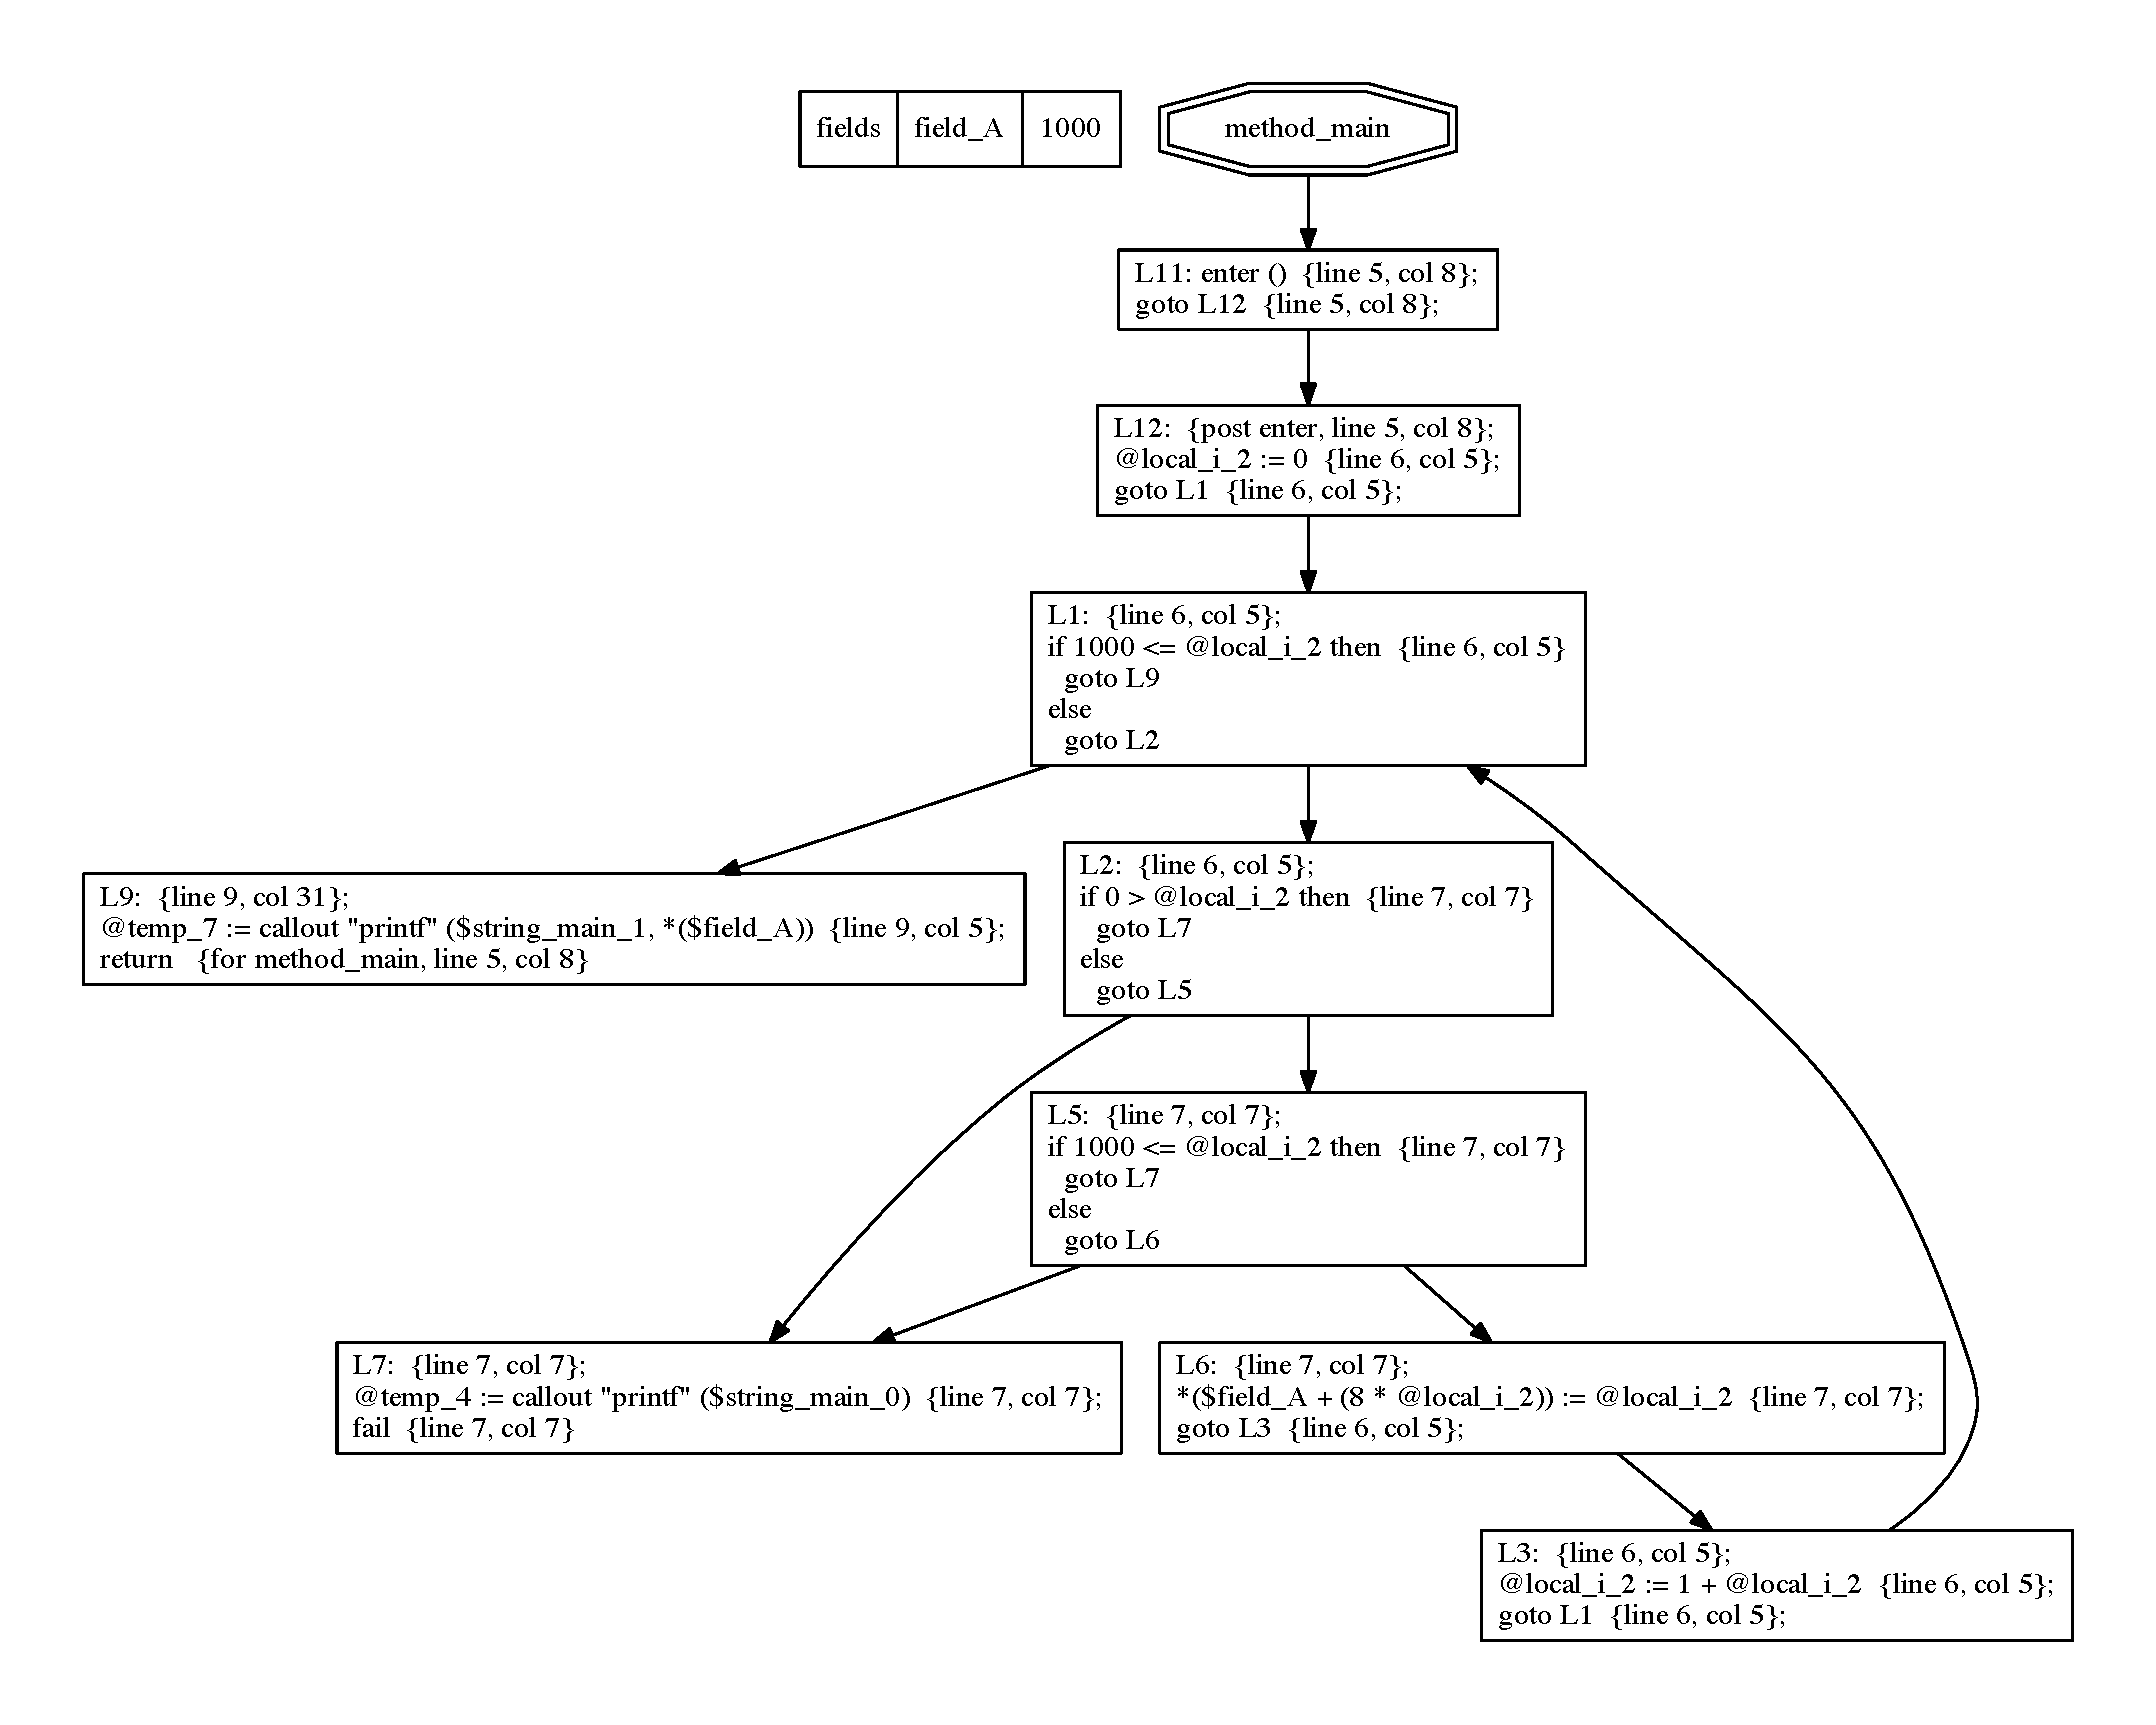
\includegraphics[width=500px]{graphs/before_parallel}\\
The Mid-IR before parallelization.
\end{center}

\begin{center}
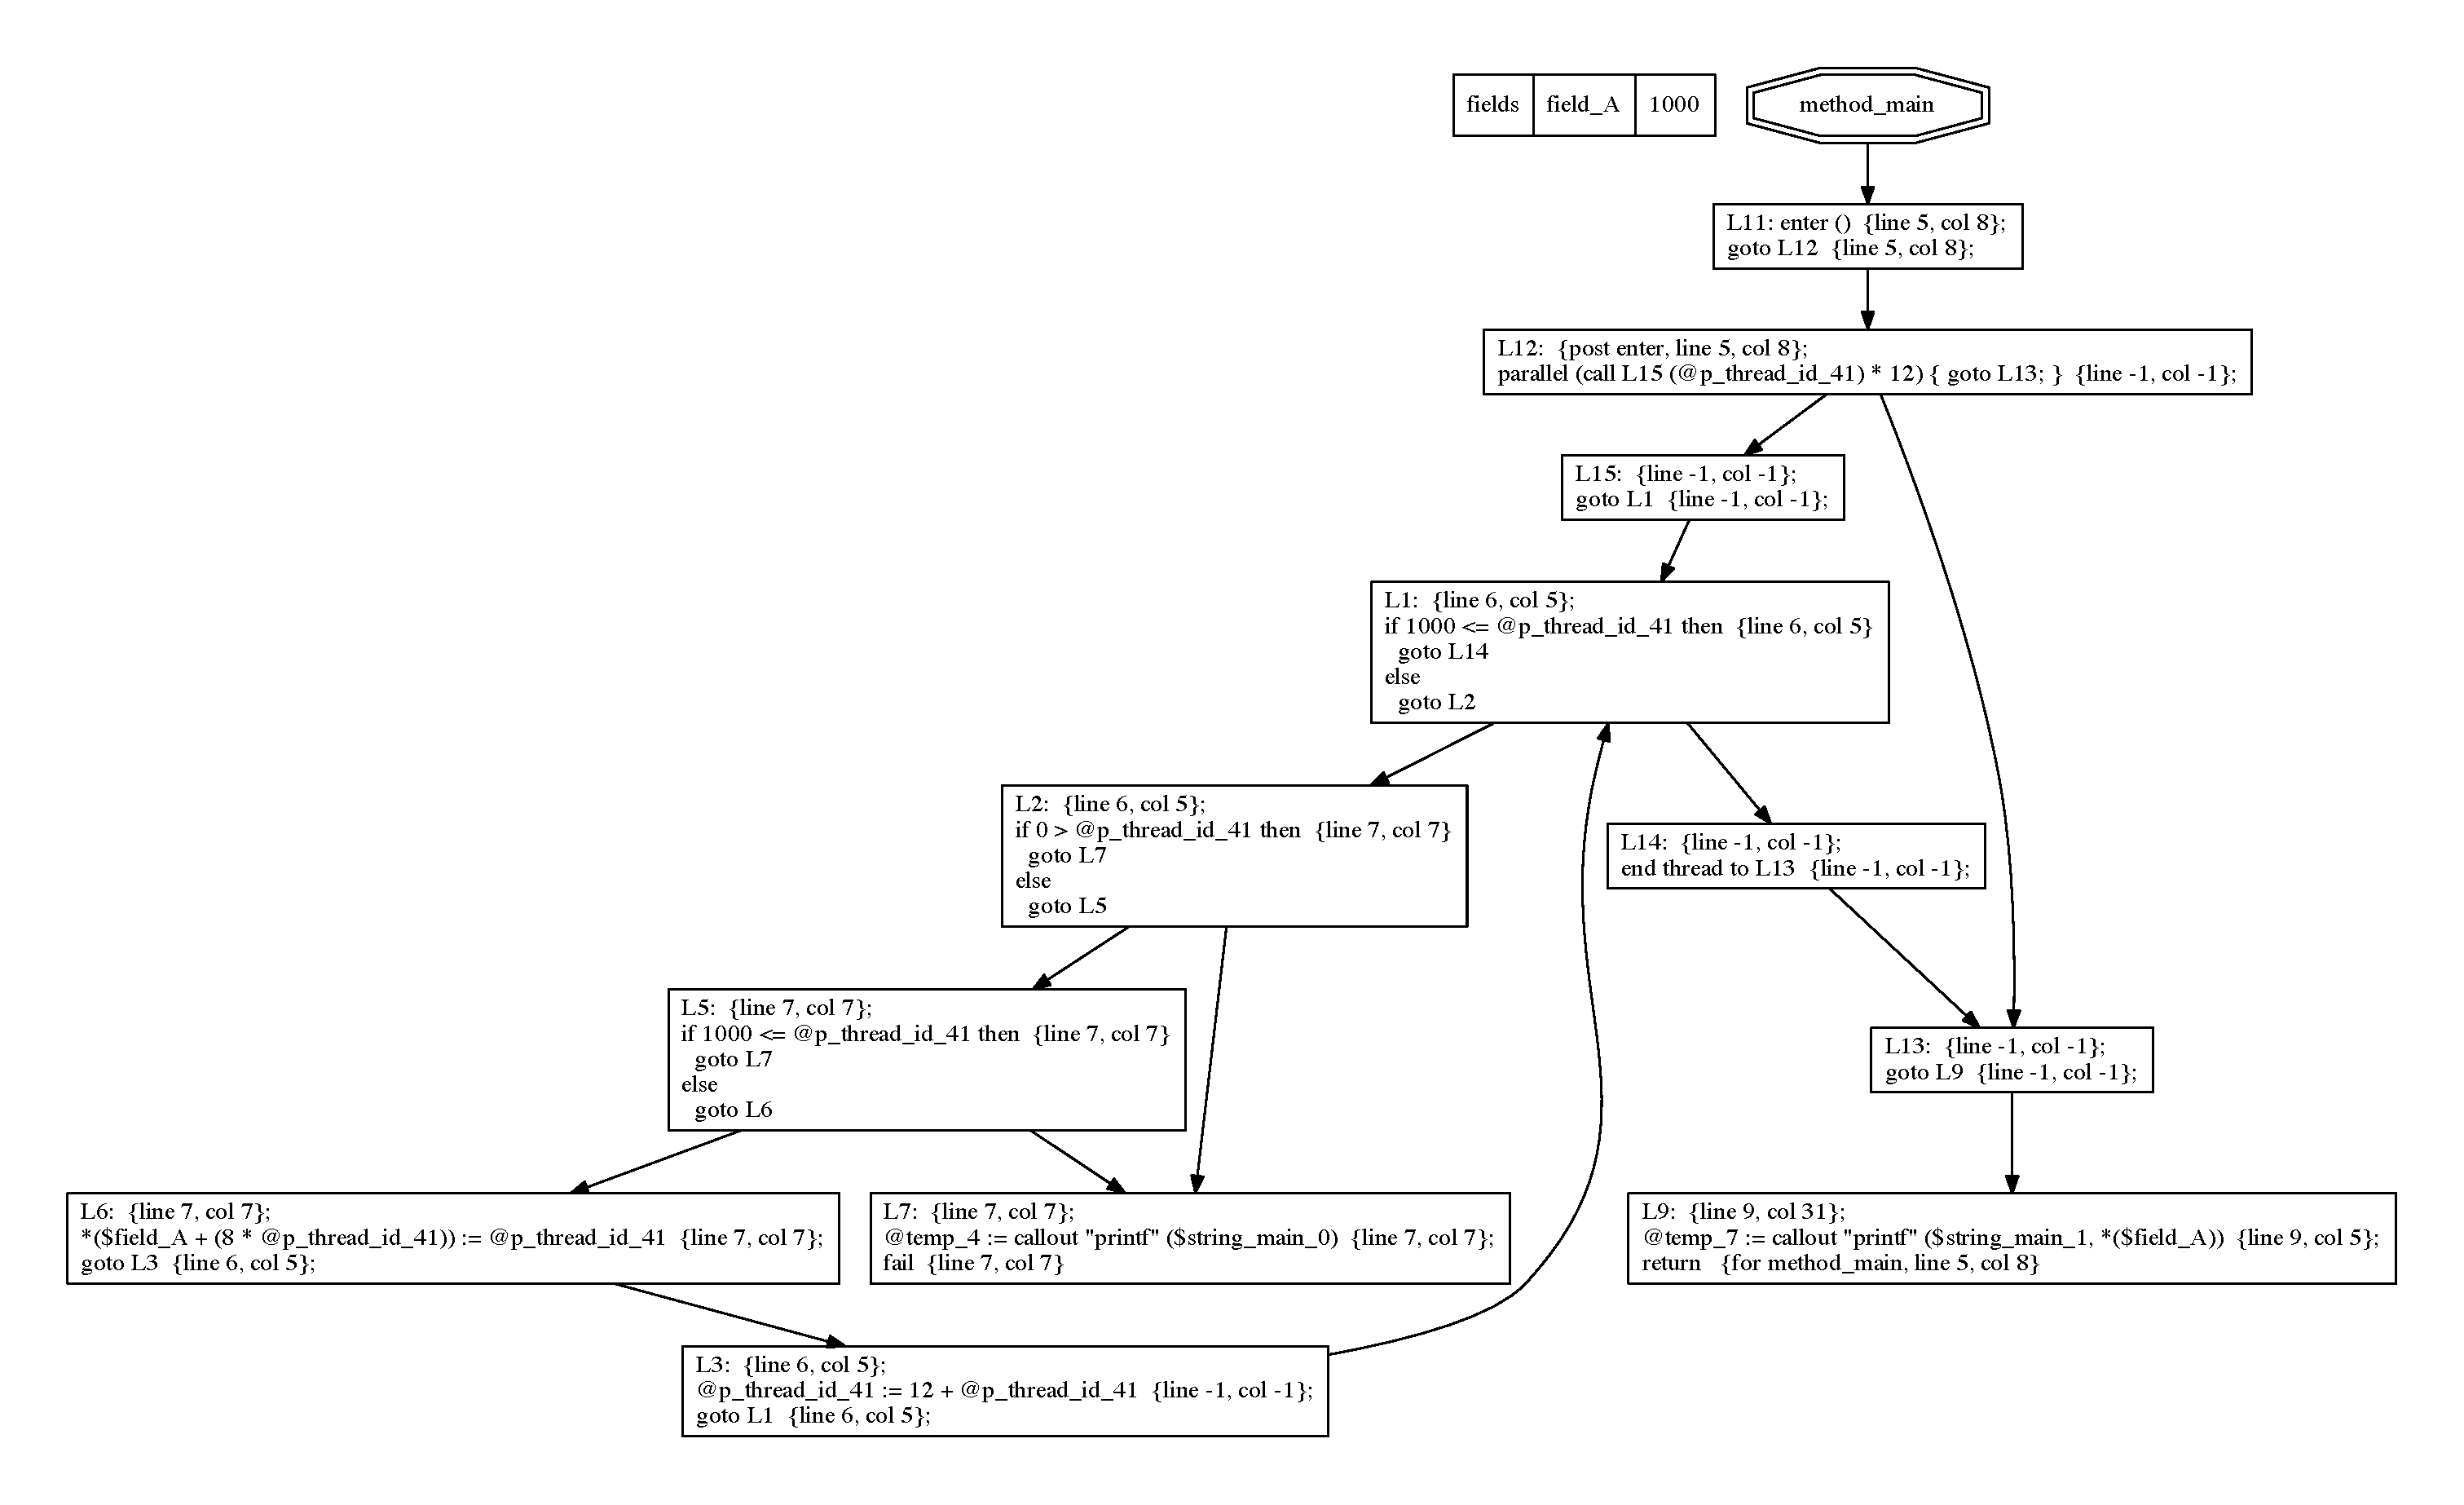
\includegraphics[width=500px]{graphs/after_parallel}\\
The Mid-IR after parallelization. 
\end{center}

Ultimately, with a loop cost threshold of about 1000000, we found
that parallelization could provide up to a 75\% speedup on
specifically designed tests (such as large matrix multiply). On test cases
that were almost exclusively parallel loops, the parallelizer could
produce speedup results close to the number of cores on the target
machine. 

% add some graphs

\section{Loop Invariant Code Motion}

Loop Invariant Code Motion (LICM) moves loop-invariant instructions
out of loops so they execute less frequently. The optimization is
important because some compiler-generated instructions are
loop-invariant and get repeated over and over, which is clearly a
waste of resources. The implementation consists of a dataflow analysis
and a non-local rewrite function: the rewrite function uses the State
monad to ensure that instructions only get moved once.

\section {Test Plan}
\label{sec:test}

Our test plan consisted of several redundant factors to increase the
probability that we catch any errors with our compiler. First, our
test suite includes a set of shell scripts that make use of every test
we've written inside a certain ``testing directory''. We also
implemented a ``Mid-IR to C'' compiler that produces valid C code from
a valid decaf program's middle IR and uses GCC to produce the expected
output. Finally, to test correctness of our compiler even further, we
implemented a complex and ``Real'' decaf program, which in our case is a
VM for a very simple stack-based programming language.

\subsection {Testing Scripts}

All the tests from each stage have been compiled into a single
directory with a single testing script. This script runs the test,
and if that test fails, it runs the Mid-IR to C converter with no
optimizations to determine whether the problem is a result of
optimizations or a result of code generation. 

\subsection {Mid-IR to C Converter} 

The Mid-IR to C converter converts from our middle IR to C. The Mid-IR
preserves the function call abstraction, but not internal control
flow. The C code is human readable, and enables us to see the results
of programs before we do register allocation and code generation.

\section {Odering of Optimizations} 
\label{sec:order}

Optimizations were split between optimizations that operated at the
Mid-IR level and optimizations that operated at the Assembly
level. The ordering of optimizations at the Mid-IR level, derived in
part from Muchnick and in part from experimenting with what actually
caused positive changes to the code, was as follows: 

\begin{itemize}

\item Constant Propagation immediately followed by Algebraic
  Simplification. 

\item Initial Tail Call Optimizations 

\item Conditional Assignment Elimination First Pass

\item Dead Code Elimination

\item Conditional Assignment Elimination Second Pass

\item Unreachable Code Elimination

\item Constant Propagation and Algebraic Simplification Second Pass

\item Global CSE (with flattening of the mid-ir)

\item Global Copy Propagation

\item Constant Propagation and Algebraic Simplification Third Pass

\item Dead Code Elimination Second Pass

\item Unflattening of the Mid-IR

\item Dead Code Elimination Third Pass

\item Tail Call Second Pass

\item Parallelization 

\item Constant Propagation and Algebraic Simplification Fourth Pass

\item Copy Propagation Second Pass

\item Dead Code Elimination Fourth Pass

\item Unreachable Code Elimination Second Pass

\item Dead Code Elimination Fifth Pass

\end{itemize}

Some highlights include the fact that Dead Code Elimination is run
after nearly every optimization because it was often easier to let
other optimizations introduce new code assuming Dead Code Elimination
will take care of the redundant code later. After the Mid-IR
optimizations, the Mid-IR is converted to a Low-IR comprised of
assembly instructions. As explained above, the code generator is
relatively smart about choosing correct assembly
instructions to perform certain operations. After code generation, a
series of optimizations is performed on the Low-IR. The ordering of
these optimizations is as follows: 

\begin{itemize}

\item Register Allocation 

\item Dead Code Elimination for Assembly 

\item Spill Location Allocation (Essentially Register Allocation for
  the spill locations)

\item Assembly-Level Constant and Copy Propagation 

\item Dead Code Elimination for Assembly Second Pass

\item Assembly-Level Branch Optimization (including Unreachable Code Elimination)

\end{itemize}

Again, the ordering of these optimizations was derived in part from
Muchnick and in part from experimenting with what appeared to be
useful. 

\section{Conclusion}

In conclusion, we feel we learned a lot about the world of compiler
design along with a whole slew of general CS knowledge. A few things
we took away from this project were the fact that Haskell is a very
useful and powerful language for designing compilers, designing an
optimizing compiler for even a very simple language spec can be
exceedingly complex, loop parallelization is one of the most powerful
optimizations a compiler can perform when given the right
circumstances, and large team projects are considerably more managable
when the given tasks are highly parallelizable, just like loops. 

\end{document}
